\documentclass[12pt,a4paper]{article}
\usepackage[utf8]{inputenc}
\usepackage[russian]{babel}
\usepackage{url}
\usepackage{amsmath}
\usepackage{amsfonts}
\usepackage{amssymb}
\usepackage[left=2cm,right=2cm,top=2cm,bottom=2cm]{geometry}
\newcommand{\e}{\varepsilon}
\renewcommand{\b}{\beta}
\newcommand{\hb}{\hat{\b}}
\newcommand{\hs}{\hat{\sigma}}
\usepackage{graphicx}
\begin{document}

5-1-1 Гомоскедастичность

\url{http://www.youtube.com/watch?v=zp2WTLxFuW8}

0:16 исправить заголовок лекции (который по центру экрана) на <<Гетероскедастичность>>. Заголовок фрагмента (тот что на синей полосе) оставить <<Гомоскедастичность>>


0:23 написать каким-нибудь стилизованным под старину шрифтом:

Разноразбросие

0:28 заголовок <<Гомоскедастичность>> исправить на <<Условная гомоскедастичность>>

0:31 исправить формулу на

$Var(\e_i|X)=E(\e_i^2|X)=\sigma^2$

0:46 добавить ниже формулы: 

<<Условная гетероскедастичность>>   (синий заголовок, как <<Условная гомо...>>)

* В реальности иногда оказывается, что

$Var(\e_i|X)=E(\e_i^2|X) \neq const$

1:06 изменяем появляющуюся фразу на 

Что происходит, если предпосылка условной гомоскедастичности нарушена?

1:18 убираем старые надписи, появляются только новые четыре надписи с буллетами (написаны верно)

* Условная гомо...

* Условная гетеро...

* Безусловная гомо...

* Безусловная гетеро...

5-1-2 Условная гетероскедастичность 

\url{http://www.youtube.com/watch?v=E4P57J6Dp8M}

ок

5-1-3 Безусловная гетероскедастичность

\url{http://www.youtube.com/watch?v=znxPMtkEJaI}

ок

5-1-4 Последствия гетероскедастичности для малых выборок

\url{http://www.youtube.com/watch?v=5ZLCCxwPQdA}

0:16 исправить заголовок лекции (который по центру экрана) на <<Гетероскедастичность>>


0:25 Заменяем появляющиеся надписи на следующие:

Случайная выборка

* Безусловной гетероскедастичности не бывает

* Когда ожидать наличие условной гетероскедастичности?

1:31 добавляем ниже <<ответ>> на вопрос :

- при наличии <<размера>> у объектов

2:48 добавляем ниже второй <<ответ>> на вопрос:

- практически всегда в случайной выборке


3:01 изменяем заголовок на <<Кроме гетероскедастичности всё ок>>

3:07 убрать остаток от переноса в слове <<стохастическими>>

3:12 очищаем экран, оставляя только заголовок <<Кроме гетероскедастичности всё ок>>

3:12 добавляем пункт

* Строгая экзогенность, $E(\e_i|X)=0$

3:22 добавляем пункт

* Некоррелированность ошибок, $Corr(\e_i,\e_j|X)=E(\e_i \e_j|X)=0$

3:40 добавляем пункт

* $n>k$

3:49 добавляем пункт 

* С вероятностью 1 нет линейно зависимых регрессоров

4:04 добавляем пункт

* Наблюдения --- случайная выборка

4:49 добавляем пропущенное <<равно>> во второй формуле, должно быть

$\widehat{Var}(\hb|X)=\frac{RSS}{n-k}(X'X)^{-1}$

5:45 убрать скобки в третьем пункте, чтобы он выглядел:

* асимптотические свойства без предположения о нормальности $\e$

6:30 справа от <<линейность по $y$>> появляется крупная зеленая галочка. Комментарий для монтажеров: идет перечисление старых свойств. Часть из них сохраняется, их надо отмечать зеленой галочкой справа, часть из них нарушается, их надо отмечать красным крестом справа.

6:43 вместо текущей добавки добавляем такое второе свойство:

* Несмещённость

$E(\hb|X)=\beta$, $E(\hb)=\beta$

7:00 справа от второго свойства <<Несмещённость>> появляется крупная зеленая галочка

7:26 вместо текущей третьей и четвертой добавки добавляем такое третье свойство:

* Оценки эффективны среди линейных несмещённых

7:54 справа от третьего свойства <<Оценки эффективны...>> появляется крупный красный крест

5-1-5

\url{http://www.youtube.com/watch?v=lDdcaMTO_JA}


0:16 исправить заголовок лекции (который по центру экрана) на <<Гетероскедастичность>>

0:27 появляется пункт (сейчас перепутан порядок появления пунктов)

* $t=\frac{\hat{\beta}_j-\beta_j}{se(\hat{\beta}_j)} | X \sim t_{n-k}$

1:03 справа от формулы $t=...$ появляется крупный красный крест

1:21 добавляется пункт

* $\frac{RSS}{\sigma^2} |X \sim \chi^2_{n-k}$

1:42 справа от формулы $\frac{RSS}{\sigma^2} |X \sim \chi^2_{n-k}$ появляется крупный красный крест

2:02 добавляется пункт

* $F=\frac{(RSS_R-RSS_{UR})/r}{RSS_{UR}/(n-k)} \sim F_{r,n-k}$

2:45 справа от формулы $F=...$ появляется крупный красный крест

3:36 исправить появляющийся заголовок на <<Асимптотические свойства>>

3:49 добавить буллет перед выезжающим пунктом $\hb \to \beta$

4:00 справа от пункта $\hb \to \beta$ появляется крупная зелёная галочка

4:20 второй пункт появляется ниже (а не справа) первого с буллетом:

* $\frac{RSS}{n-k} \to \sigma^2$

4:28 справа от пункта $\frac{RSS}{n-k} \to \sigma^2$ появляется зелёная галка

4:50 добавить буллет слева от формулы:

* $t=\frac{\hat{\beta}_j-\beta_j}{se(\hat{\beta}_j)} \to N(0,1)$

5:18 справа от формулы $t=...$ появляется красный крест

5:47 добавить буллет слева от формулы:

* $\frac{RSS_R-RSS_{UR}}{RSS_{UR}/(n-k)} \to \chi^2_r$

6:29 справа от формулы $... \to \chi^2_r$ появляется красный крест


5-1-6 Обнаружение гетероскедастичности и стандартные ошибки Уайта

\url{http://www.youtube.com/watch?v=dlUzgxuoahA}

0:16 исправить заголовок лекции (который по центру экрана) на <<Гетероскедастичность>>

1:59 под заголовком <<Что делать?>> расположить:

* Вместо старых стандартных ошибок $se(\hb_j)$ использовать другие стандартные ошибки $se_{HC}(\hb_j)$. 

HC --- heteroskedasticity consistent, устойчивые к гетероскедастичности

- $se(\hb_j)$ --- корни из диагональных элементов матрицы $\widehat{Var}(\hb|X)$

- $se_{HC}(\hb_j)$ --- корни из диагональных элементов матрицы $\widehat{Var}_{HC}(\hb|X)$

2:05 новый заголовок с новым текстом под ним пока не появляется, пока висит старый текст

2:23 только сейчас стираем старый текст и появляется новый  под заголовком <<Робастная...>>. В 2:23 сразу появляется:

Робастная (устойчивая) к гетероскедастичности оценка ковариационной матрицы

* Вместо $\widehat{Var}(\hat{\beta}|X)=\frac{RSS}{n-k}(X'X)^{-1}$ 

использовать $\widehat{Var}_{HC}(\hat{\beta}|X)=(X'X)^{-1}X'\hat{\Omega}X(X'X)^{-1}$

- Уайт, 1980, HC0: 

$\hat{\Omega}=diag( \hat{\varepsilon}_1^2, \ldots, \hat{\varepsilon}_n^2 )$

4:49 добавляем буллет слева от каждой из трёх формул, вместо зачеркивания формулы ставим красный крест справа от формулы

5:04 добавляем буллет слева от формулы, справа от формулы рисуем зелёную галку

5:48 исправляем заголовок на <<Когда следует использовать робастные оценки дисперсии?>>

5:50 сокращаем ответ до 

Как только есть случайная выборка и объекты могут быть разного <<размера>>

7:13 график пока не показывать (а показать оба со словами <<Перед Вами два графика>>

7:54 показать оба графика, на графиках увеличить шрифт, два пункта слева от графиков убрать с появлением графиков

8:43 под заголовком появляется только названия двух тестов:

* Тест Уайта

* Тест Голдфельда-Квандта

9:00 убираем из заголовка слово <<начало>> и добавляем два пункта под:

Тест Уайта

* Асимптотический

* Не требуется нормальность остатков

9:17 стираем надписи под заголовком и появляется нумерованный список

1. Оценить основную регрессию, получить $\hat{\varepsilon}_i$

2. Оценить вспомогательную регрессию:

$\hat{\varepsilon}^2_i = \gamma_1 + \gamma_2 z_{i2} + \ldots + \gamma_{i,m} z_{im}+ u_i$

$z_{i2}$, \ldots, $z_{im}$ --- факторы, определяющие форму гетероскедастичности

3. Посчитать статистику Уайта

$LM=nR^2_{aux}$


10:12 название оставляем просто <<Тест Уайта>>, меняем текст под названием

Тест Уайта


* Если верна

$H_0$: условная гомоскедастичность, $Var(\e_i|X)=\sigma^2$

* То асимптотически $LM\sim \chi^2_{m-1}$

$m$ --- число коэффициентов во вспомогательной регрессии:

$\hat{\varepsilon}^2_i = \gamma_1 + \gamma_2 z_{i2} + \ldots + \gamma_{i,m} z_{im}+ u_i$

10:46 появляется график, блок <<подписи на графике>> внизу справа экрана убираем полностью, на графике меняем подписи и убираем закраску, должно быть так, 

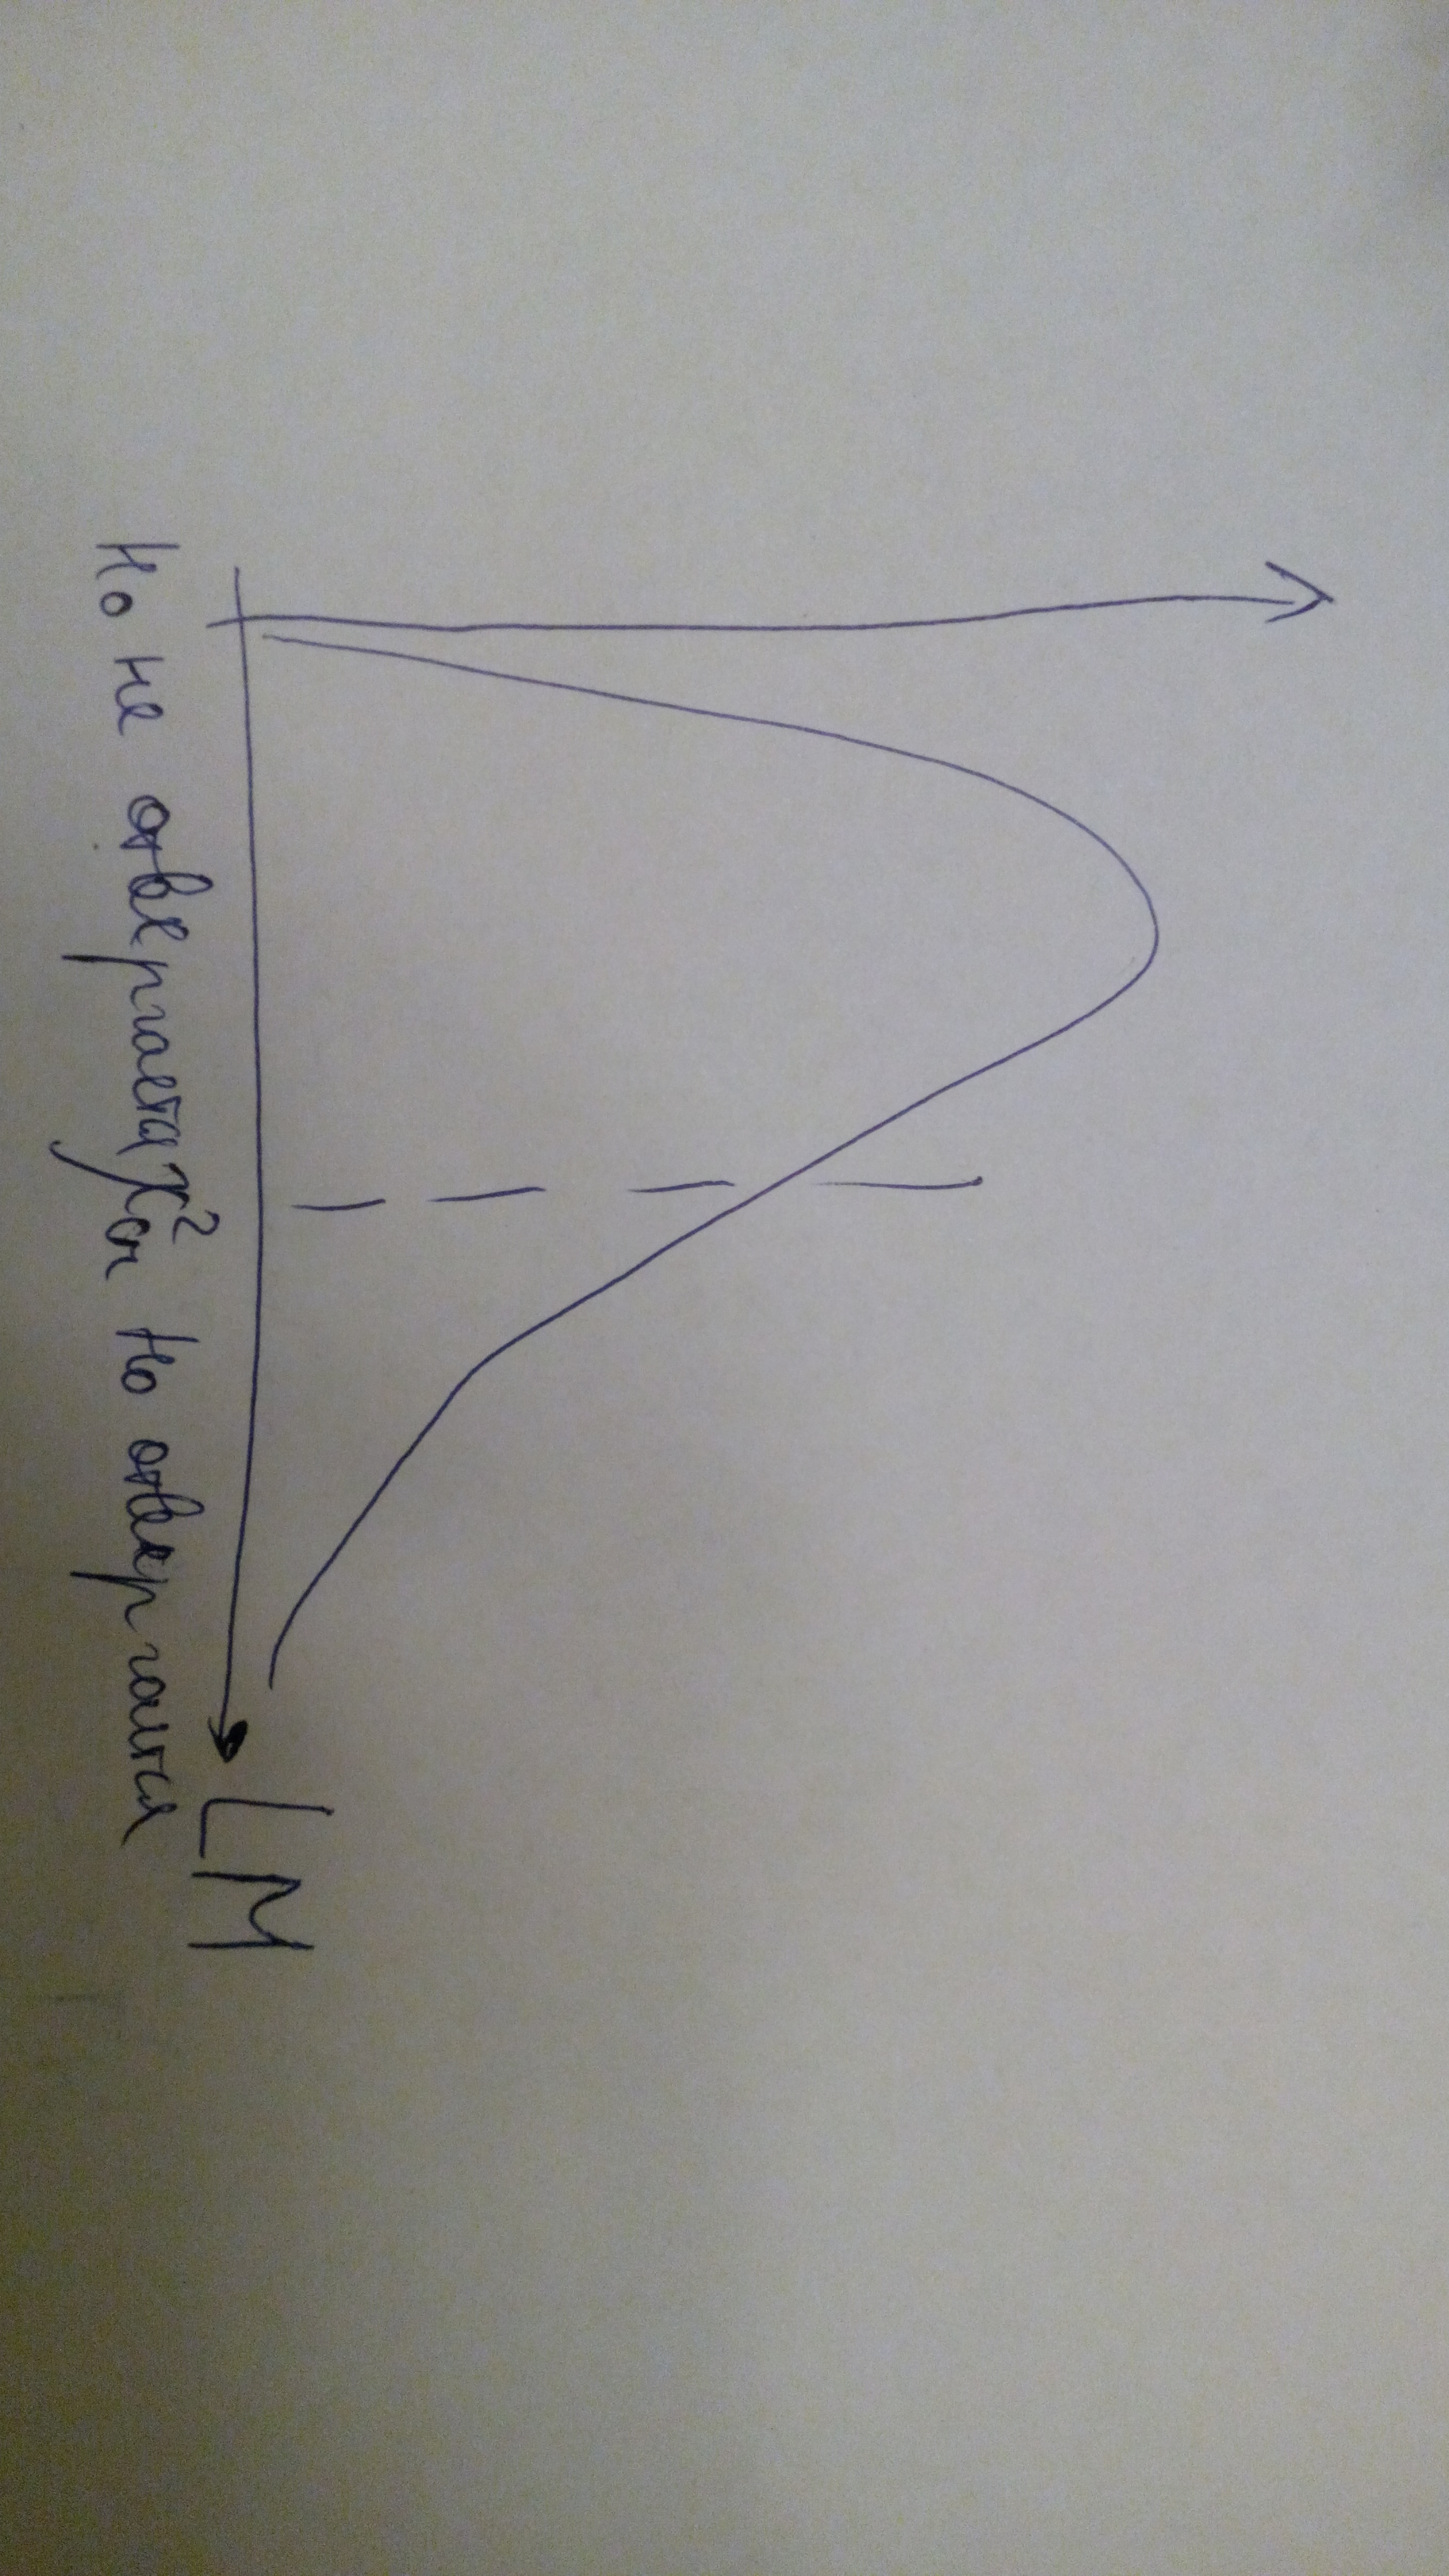
\includegraphics[scale=0.1, angle=90]{white_test.jpg} 

Если почерк плохой, то под осью должно быть:

$H_0$ не отвергается  \hspace{1cm} $\chi^2_{cr}$ \hspace{1cm} $H_0$  отвергается  

5-1-7 пропущен фрагмент! должно быть видео у доски про тест Уайта

если его нет, то надо переснять

5-1-8  

\url{http://www.youtube.com/watch?v=ohD-vYa3Sog}

0:16 исправить заголовок лекции (который по центру экрана) на <<Гетероскедастичность>>

0:29 первый пункт из трёх исправить на:

* Есть переменная, от которой предположительно монотонно зависит условная дисперсия ошибок

(остальный два пункта верно)

0:48 превращаем список с буллетами в нумерованный список, т.е. сначала появляется

1. Сортируем наблюдения по предполагаемому убыванию условной дисперсии

1:36 буллет меняем на цифру 2, добавляем слово например:

2. Выкидываем часть наблюдений посередине (например, 20\%)

2:10 буллет меняем на цифру 3 и начинаем с заглавной буквы

3. Оцениваем исходную модель отдельно по первым и по последним наблюдениям

2:38 добавляем пункт

4. Из двух регрессий получаем $RSS_1$, $RSS_2$

2:57 добавляем пункт

5. Считаем $F=\frac{RSS_1/(n_1-k)}{RSS_2/(n_2-k)}$

3:26 на слайде должно быть:

Тест Голдфельда-Квандта (заголовок, синим)

* Если верна

$H_0$: условная гомоскедастичность, $Var(\e_i|X)=\sigma^2$

* То $F=\frac{RSS_1/(n_1-k)}{RSS_2/(n_2-k)} \sim F_{n_1-k,n_2-k}$

$n_1$ --- число наблюдений в <<верхней>> части выборки

$n_2$ --- число наблюдений в <<нижней>> части выборки

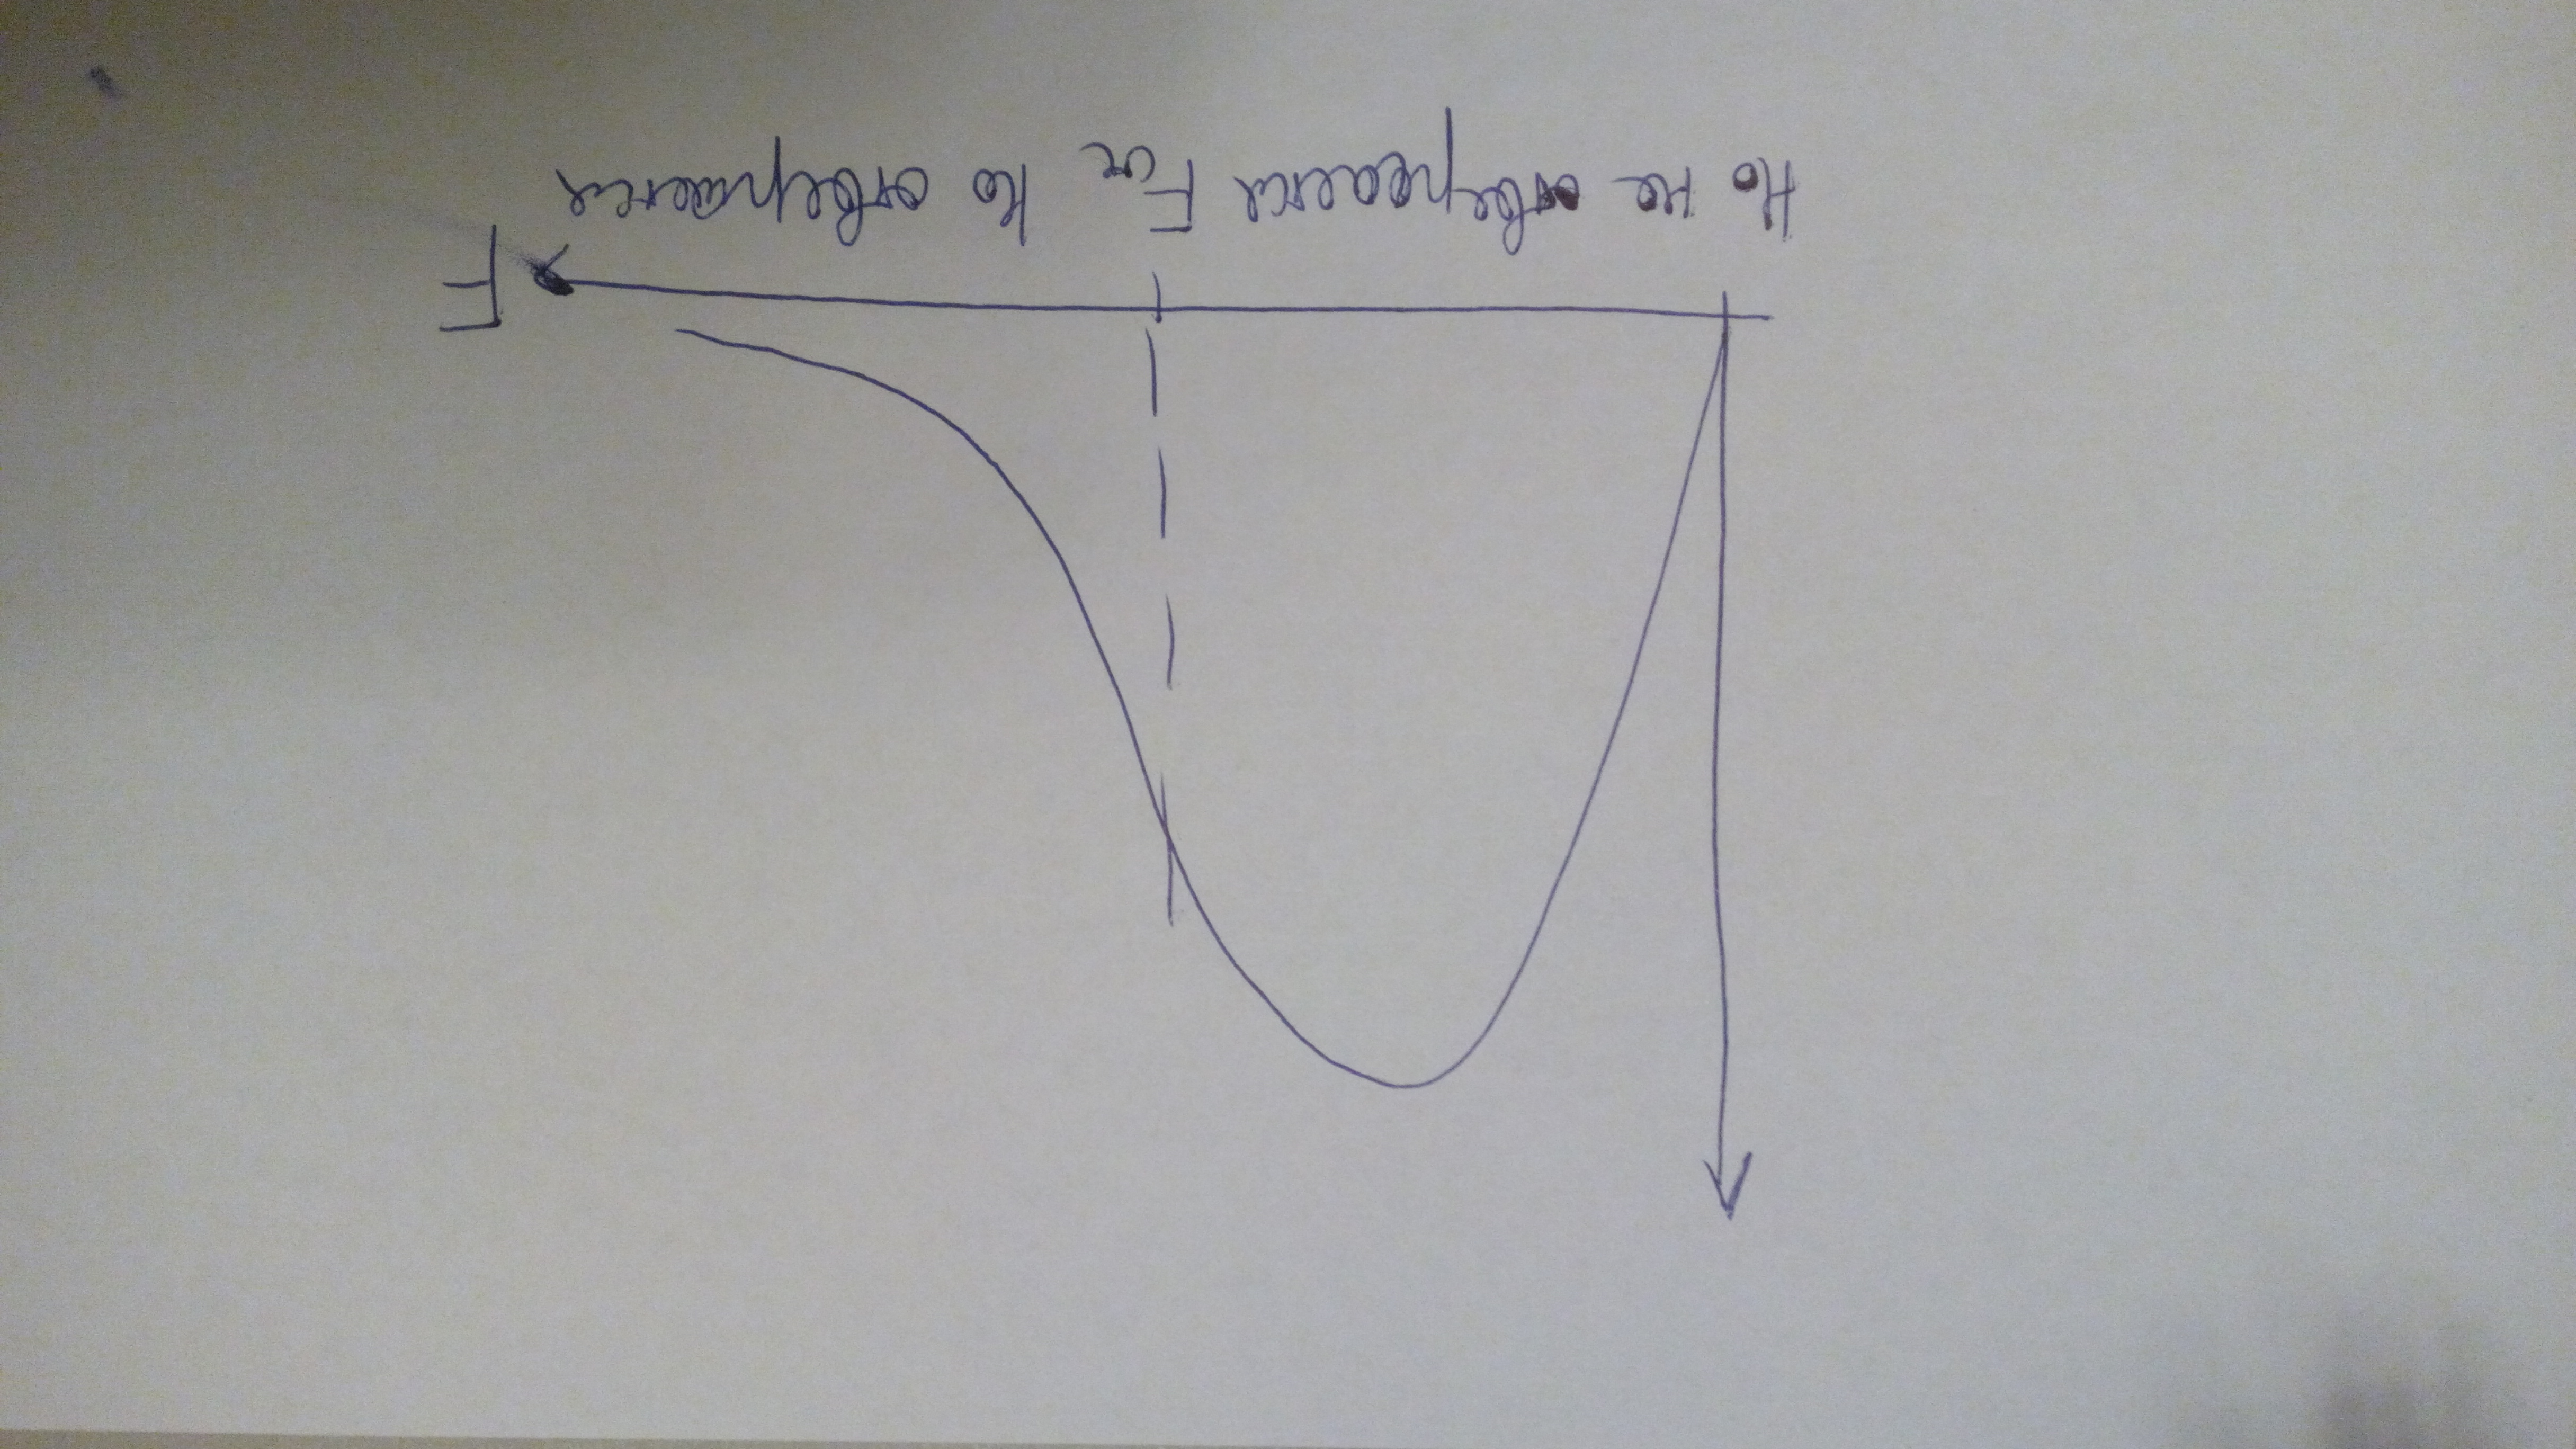
\includegraphics[scale=0.1, angle=180]{goldfeld_test.jpg} 

Если почерк плохой, то под осью должно быть:

$H_0$ не отвергается  \hspace{1cm} $F_{cr}$ \hspace{1cm} $H_0$  отвергается 

4:33 --- до конца фрагмента --- переснять доску из-за невидимого маркера

5-1-9 

\url{http://www.youtube.com/watch?v=2oTzEKvV4n4}

0:16 исправить заголовок лекции (который по центру экрана) на <<Гетероскедастичность>>

0:25 исправить второй пункт на (сделать $n$ синим и вставить $se_{HC}(\hb)$)

* Новые стандартные ошибки $se_{HC}(\hb)$ исправляют ситуацию при больших $n$

от 2:54 до конца переснять из-за невидмого маркера (модель с заданной формой гетероскедастичности)

0:48 пока ещё новые пункты не появляются

1:14 дополнительно появляются только два пункта (попутно убрать дефис и вставить $\hb$):

* Да, надо смириться с тем, что оценки $\hb$ неэффективны

* Мы довольны несмещенностью, состоятельностью $\hb$ и возможностью проверять гипотезы

2:00 заголовок остаётся, четыре пункта стираются, появляется пятый (без буллета):

Для получения эффективных оценок нужно точно понимать как устроена гетероскедастичность. Это большая редкость.

5-1-10 

\url{http://www.youtube.com/watch?v=O4yA7lXBE5c}

от начала до 6:26  --- переснять

6:35  немного исправить первые два пункта: в первый пункт вставить формулу и убрать разрыв в слове <<предпосыл ки>>, во втором добавить про выборку, чтобы вышло:

* Мы рассмотрели ситуацию нарушения предпосылки условной гомоскедастичности, $Var(\e_i|X)=\sigma^2$ 

* Гетероскедастичность в случайной выборке почти всегда есть

5-2-1 Написание функций в R

\url{http://www.youtube.com/watch?v=jwVgJVPUKpw}

0:16 исправить заголовок лекции (который по центру экрана) на <<Гетероскедастичность>>


5-2-2 Написание циклов в R

\url{http://www.youtube.com/watch?v=XyqbFLRQxGQ}

0:16 исправить заголовок лекции (который по центру экрана) на <<Гетероскедастичность>>

5-2-3 переснять из-за пакета bstats

5-2-4 Доверительные интервалы при гетероскедастичности

\url{http://www.youtube.com/watch?v=Vl5dKXFyLEc}

0:16 исправить заголовок лекции (который по центру экрана) на <<Гетероскедастичность>>

5-2-5 переснять из-за пакета bstats

\end{document}